\section{Graftyper}
En graf er, som tidligere nævnt, en struktur med knuder og kanter. Den er givet ved definitionen:
\begin{defn}
[Graf] 
En graf $G=(V,E)$ består af $V$, en mængde af knuder, hvor $V\neq0$, og en mængde af kanter; $E \subseteq \{\{u;v\}|u,v \in V\}$.
\end{defn}
Det fremgår af definitionen, at en graf ikke kan have nul knuder, men en lignende afgrænsning i den anden ende eksisterer ikke. Der kan dermed være uendeligt mange knuder. På samme måde gælder det for kanter, at der kan være mellem nul og uendeligt. Hvis mindst et af disse tilfælde gør sig gældende, kaldes det en uendelig graf. Ellers kaldes det en endelig graf, og det er denne type, som vi beskæftiger os med i projektet.
Ydermere, ses det i definitionen, at hver kant forbinder én eller to knuder. For en simpel graf gælder det, at ingen kanter forbinder et punkt med sig selv. Der må altså ikke være løkker. Derudover forbindes to knuder med højst én kant.

\begin{figure}[H]
\centering
	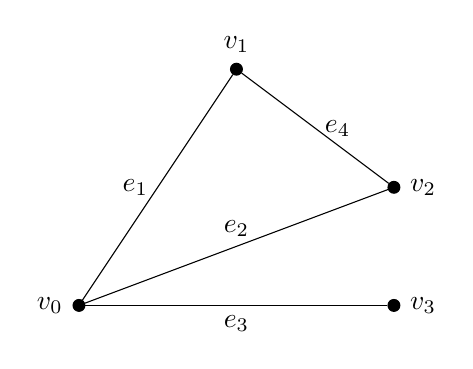
\begin{tikzpicture}

      \tikzset{enclosed/.style={draw, circle, inner sep=0pt, minimum size=.15cm, fill=black}}
%% Vertices
      	\node[enclosed, label={left: $v_0$}] (v0) at (0,0) {};
      	\node[enclosed, label={above: $v_1$}] (v1) at (2,3) {};
    	\node[enclosed, label={right: $v_2$}] (v2) at (4,1.5) {};
  	    \node[enclosed, label={right: $v_3$}] (v3) at (4,0) {};
%Edges
		\path (v0) edge node[midway, left] {$e_1$} (v1);
		\path (v0) edge node[midway, above] {$e_2$} (v2);
		\path (v0) edge node[midway, below] {$e_3$} (v3);
		\path (v1) edge node[midway, right] {$e_4$} (v2);

	\end{tikzpicture}
	\caption{En simpel graf}
	\label{fig.simpel}
\end{figure}



I kontrast til den simple graf finder vi multigrafen. For denne type graf skal der være flere kanter, der forbinder det samme sæt knuder. Der må stadig ikke optræde løkker.

\begin{figure}[H]
\centering
	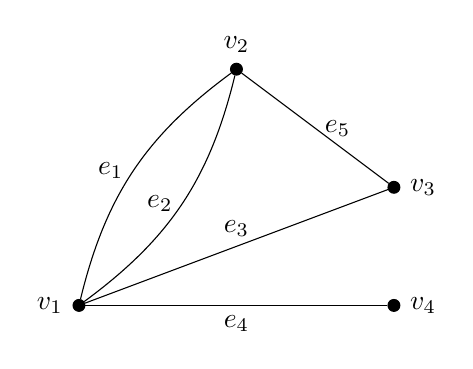
\begin{tikzpicture}

      \tikzset{enclosed/.style={draw, circle, inner sep=0pt, minimum size=.15cm, fill=black}}
%% Vertices
      	\node[enclosed, label={left: $v_1$}] (v1) at (0,0) {};
      	\node[enclosed, label={above: $v_2$}] (v2) at (2,3) {};
    	\node[enclosed, label={right: $v_3$}] (v3) at (4,1.5) {};
  	    \node[enclosed, label={right: $v_4$}] (v4) at (4,0) {};
%Edges
		\path (v1) edge [bend right=20] node[midway, left] {$e_2$} (v2);
		\path (v2) edge [bend right=20] node[midway, left] {$e_1$} (v1);
		\path (v1) edge node[midway, above] {$e_3$} (v3);
		\path (v1) edge node[midway, below] {$e_4$} (v4);
		\path (v2) edge node[midway, right] {$e_5$} (v3);

	\end{tikzpicture}
	\caption{En multigrafgraf}
	\label{fig.multi}
\end{figure}


I eksemplet ovenfor ses det, at to kanter forbinder et sæt knuder ($v_{0},v_{1}$). Hvis en graf, modsat de to allerede nævnte, indeholder mindst én løkke, kaldes det en pseudograf. Dog er alle ikke-orienterede grafer pseudografer, da det kun kræves, at de kan indeholde løkker og/eller flere kanter, der forbinder samme knuder. Vi ser i eksemplet herunder, at der er to kanter, der forbinder $v_{0}$ og $v_{1}$, og der er en løkke ved $v_{3}$.

\begin{figure}[H]
\centering
	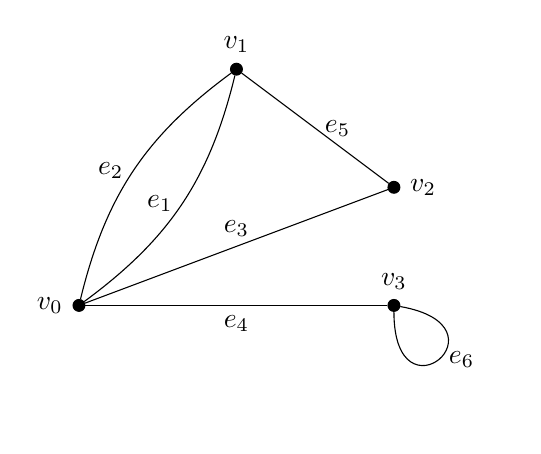
\begin{tikzpicture}[every loop/.style={}]
      \tikzset{enclosed/.style={draw, circle, inner sep=0pt, minimum size=.15cm, fill=black}}
%% Vertices
      	\node[enclosed, label={left: $v_0$}] (v0) at (0,0) {};
      	\node[enclosed, label={above: $v_1$}] (v1) at (2,3) {};
    	\node[enclosed, label={right: $v_2$}] (v2) at (4,1.5) {};
  	    \node[enclosed, label={above: $v_3$}] (v3) at (4,0) {};
%Edges
		\path (v0) edge [bend right=20] node[midway, left] {$e_1$} (v1);
		\path (v1) edge [bend right=20] node[midway, left] {$e_2$} (v0);
		\path (v0) edge node[midway, above] {$e_3$} (v2);
		\path (v0) edge node[midway, below] {$e_4$} (v3);
		\path (v1) edge node[midway, right] {$e_5$} (v2);
		\path (v3) edge [out=270,in=350,looseness=35] node[right] {$e_6$} (v3);
	\end{tikzpicture}
	\caption{En pseudograf med et loop}
	\label{fig.pseudo}
\end{figure}



\subsection{Orienterede grafer og ikke-orienterede grafer}
En anden typisk grafopdeling er opdelingen i orienterede og ikke-orienterede grafer. De grafer, vi har kigget på indtil videre, er ikke-orienterede grafer. For en orienteret graf gælder det, at grafens kanter er retningsbestemte. Dette er ofte illustreret med pile. Den har dermed en startknude og en endeknude. Disse grafer er defineret ved:

\begin{defn}
[Orienteret graf] 
En orienteret graf $G=(V,E)$ består af $V$, et sæt knuder, hvor $V\neq0$, og et sæt orienterede kanter, $E$. Hver orienterede kant forbinder et sæt knuder $(u,v)$, hvor startknuden $u$ er tilstødende til endeknuden $v$. 
\end{defn}

\begin{figure}[H]
\centering
	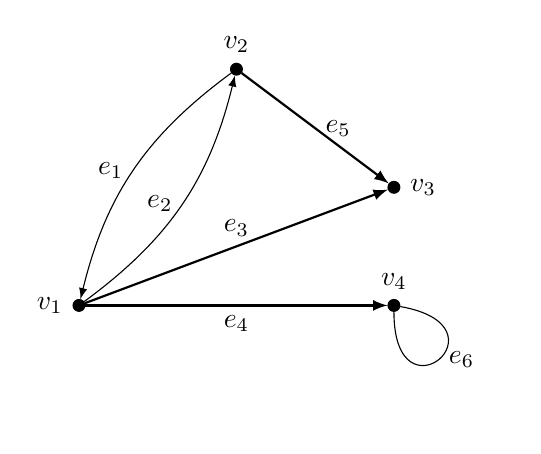
\begin{tikzpicture}[every loop/.style={}]
      \tikzset{enclosed/.style={draw, circle, inner sep=0pt, minimum size=.15cm, fill=black}}
%% Vertices
      	\node[enclosed, label={left: $v_1$}] (v1) at (0,0) {};
      	\node[enclosed, label={above: $v_2$}] (v2) at (2,3) {};
    	\node[enclosed, label={right: $v_3$}] (v3) at (4,1.5) {};
  	    \node[enclosed, label={above: $v_4$}] (v4) at (4,0) {};
%Edges
		\path[->, > = latex] (v1) edge [bend right=20] node[midway, left] {$e_2$} (v2);
		\path[->, > = latex] (v2) edge [bend right=20] node[midway, left] {$e_1$} (v1);
		\path[->, > = latex, thick] (v1) edge node[midway, above] {$e_3$} (v3);
		\path[->, > = latex, thick] (v1) edge node[midway, below] {$e_4$} (v4);
		\path[->, > = latex, thick] (v2) edge node[midway, right] {$e_5$} (v3);
		\path (v4) edge [out=270,in=350,looseness=35] node[right] {$e_6$} (v4);
	\end{tikzpicture}
	\caption{En orienteret graf}
	\label{fig:orienteret}
\end{figure}


%\ref{fig:orienteret}
%\begin{figure}[H]
%\centering
%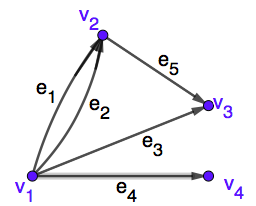
\includegraphics[scale=0.5]{fig/img/orienteret_graf.png}
%\caption{En orienteret graf}
%\label{fig:orienteret}
%\end{figure}


Der kan foruden disse to også være tale om mixede grafer, som er grafer med både orienterede og ikke-orienterede kanter. Orienterede grafer kan ligesom ikke-orienterede grafer indeholde løkker og flere kanter, der forbinder det samme sæt knuder, men hvis dette ikke er tilfældet, kaldes det en orienteret simpel graf. Hvis der derimod optræder flere kanter mellem et eller flere punktpar, kaldes det en orienteret multigraf. Den må også indeholde flere modsatrettede kanter mellem det samme knudepar. Dermed kan en kant gå fra $v$ til $u$, selvom en anden kant går fra $u$ til $v$. 

Egenskaberne for de forskellige grafer kan ses herunder:

\begin{tabular}{ |p{4cm}||p{3cm}|p{3cm}|p{2cm}|  }
 \hline
 \multicolumn{4}{|c|}{Grafer} \\
 \hline
 Type & Kanter & Flere kanter per knudepar tilladt? & Løkker tilladt\\
 \hline
 Simpel graf   & Ikke-orienteret    & Nej &   Nej\\
 Multigraf &   Ikke-orienteret & Ja   & Nej\\
 Pseudograf & Ikke-orienteret & Ja &  Ja\\
 Simpel orienteret graf    & Orienteret & Nej &  Nej\\
 Orienteret multigraf &  Orienteret  & Ja & Ja\\
 Mixet graf & Ikke-orienteret og orienteret  & Ja   & Ja\\
 \hline
\end{tabular}

Fordi kanterne i grafer med orienterede kanter er ordnede par, kan definitionen af knudens grader være antallet af kanter, der har denne knude som begyndelsesknude, eller antallet af kanter, der har denne knude som endeknude:
\begin{defn}
[Graden af en orienteret graf] 
I en graf med orienterede kanter er ind-graden, betegnet ved $deg^{-}(v)$, antallet af kanter med $v$ som deres endeknude. Ud-graden, betegnet ved $deg^{+}(v)$, er antallet af kanter med $v$ som deres startknude.
\end{defn}
Vi vil i projektet beskæftige os med orienterede grafer, da det er denne type, vi bruger til optimering af gaslageret. I vores tilfælde vil vi tildele vores orienterede kanter vægt, hvilket beskrives senere i projektet.
